\documentclass[xcolor=pst,dvipsnames]{beamer}

\newtheorem{question}{Question}
\mode<presentation>
{
  \usetheme{Madrid}

  \setbeamercovered{invisible}
}
%  \useoutertheme{shadow}

%\setbeamercolor{title}{fg=purple!80!black,bg=purple!20!white}
  \beamertemplateshadingbackground{black!50!white}{white}
  \setbeamercolor{alerted text}{fg=RoyalBlue}
  \usenavigationsymbolstemplate{}
%  \usebeamercolor[bg]{black}

  \xdefinecolor{kaustyellow}{rgb}{0.9176,0.6706,0}
  \xdefinecolor{kaustcyan}{rgb}{0.,0.6980,0.6}
  \xdefinecolor{kaustcyandark}{rgb}{0.,0.3452,0.2}
  \xdefinecolor{kaustorange}{rgb}{0.882,0.4392,0.}
  \xdefinecolor{kaustolive}{rgb}{0.7137,0.7490,0.}
%  \beamertemplateshadingbackground{kaustcyan!50!white}{kaustcyan!90!white}
%  \setbeamercolor{alerted text}{fg=kaustyellow}
  \setbeamercolor{frametitle}{fg=white,bg=kaustcyan!50!black}
  \setbeamercolor{frametitle right}{fg=white,bg=kaustcyan}
  \setbeamercolor{title}{fg=white,bg=kaustcyan!50!black}
  \setbeamercolor{normal text}{fg=kaustcyan!30!black}
 
  \usecolortheme[named=kaustcyandark]{structure}

\setbeamercolor*{palette primary}{use=structure,fg=white,bg=kaustcyan!90!black}
\setbeamercolor*{palette secondary}{use=structure,fg=white,bg=kaustorange!90!black}
\setbeamercolor*{palette tertiary}{use=structure,fg=black,bg=kaustyellow!90!black}
%\usepackage[english]{babel}
%\usepackage[latin1]{inputenc}

\setbeamercolor{item}{fg=kaustorange,bg=kaustyellow}
\setbeamercolor{item text}{fg=kaustorange,bg=kaustyellow}

%\usepackage[T1]{fontenc}
\usepackage{graphicx}
\usepackage{pstricks,pst-plot,pstricks-add}
\usepackage{pst-pdf}
\usepackage{pgf}
\usepackage{multimedia}
\usepackage{fancybox}


\title[]{"Shocking" Wave Phenomena in Periodic Materials}
\author[D. Ketcheson]{David I.~Ketcheson}

%\institute[KAUST]
%{King Abdullah University of Science \& Technology \\ (KAUST)}

\date{Nov. 4, 2010}

%  \setbeamertemplate{sidebar canvas}[vertical shading][top=red!20,bottom=yellow!30]
\begin{document}


%\newtheorem{thm}{Theorem}
%\newtheorem{dfn}{Definition}
%\newtheorem{lem}{Lemma}
%\newtheorem{rmk}{Remark}
%\newtheorem{cor}{Corollary}

%\newtheorem{proposition}{Proposition}
%\newtheorem{result}{Result}
%\newtheorem{proof}{Proof}

\newcommand{\qh}{\hat{q}}
\newcommand{\be}{\begin{equation}}
\newcommand{\ee}{\end{equation}}
\newcommand{\bq}{\mathbf{q}}
\newcommand{\bx}{\mathbf{x}}
\newcommand{\br}{\mathbf{r}}
\newcommand{\imh}{{i-\frac{1}{2}}}
\newcommand{\iph}{{i+\frac{1}{2}}}
\newcommand{\ipmh}{{i \pm \frac{1}{2}}}
\newcommand{\jph}{{j+\frac{1}{2}}}
\newcommand{\Aop}{{\cal A}}
\newcommand{\Bop}{{\cal B}}
\newcommand{\Wop}{{\cal W}}
\newcommand{\Oop}{{\cal O}}
\newcommand{\DQ}{\Delta Q}
\newcommand{\Dq}{\Delta q}
\newcommand{\Dx}{\Delta x}
\newcommand{\Dy}{\Delta y}
\newcommand{\Du}{\Delta u}
\newcommand{\bu}{\mathbf{u}}
\newcommand{\bv}{\mathbf{v}}
\newcommand{\bw}{\mathbf{w}}
\newcommand{\bU}{\mathbf{U}}
\newcommand{\bV}{\mathbf{V}}
\newcommand{\bF}{\mathbf{F}}
\newcommand{\bB}{\mathbf{B}}
\newcommand{\bk}{\mathbf{k}}
\newcommand{\Lop}{{\cal L}}
\newcommand{\Fop}{{\cal F}}
\newcommand{\Dofr}{{\cal D}(r)}
\newcommand{\Dt}{\Delta t}
\newcommand{\bbA}{\mathbf{A}}
\newcommand{\bbZ}{\mathbf{Z}}
\newcommand{\bbK}{\mathbf{K}}
\newcommand{\bbI}{\mathbf{I}}
\newcommand{\bbb}{\mathbf{b}}
\newcommand{\bbe}{\mathbf{e}}
\newcommand{\bbone}{\mathbf{1}}

\newcommand{\dx}{\Delta x}
\newcommand{\dt}{\Delta t}
%\newcommand{\half}{\frac{1}{2}} 
\newcommand{\hfp}{\hat{f}_{j+\half}}
\newcommand{\hfn}{\hat{f}_{j-\half}}
\newcommand{\aik}{\alpha_{i,k}}
\newcommand{\bik}{\beta_{i,k}}
\newcommand{\lt}{\tilde{L}}

\newcommand{\hf}{\frac{1}{2}}
%\def\half{\frac{1}{2}}
\newcommand{\fracStrut}{\rule[-1.0ex]{0pt}{3.1ex}}
\newcommand{\hfs}{\ensuremath{\frac{1}{2}}\fracStrut}
\newcommand{\scinot}[2]{\ensuremath{#1\times10^{#2}}}
\newcommand{\dee}{\mathrm{d}}
\newcommand{\dye}{\partial}
\newcommand{\diff}[2]{\frac{\dee #1}{\dee #2}}
\newcommand{\pdiff}[2]{\frac{\dye #1}{\dye #2}}
\newcommand{\Real}{\mathbb{R}}
\newcommand{\Complex}{\mathbb{C}}
% matrices
\newcommand{\m}[1]{\mathbf{#1}}
\newcommand{\mA}{\m{A}}
\newcommand{\mI}{\m{I}}
\newcommand{\mK}{\m{K}}
\newcommand{\mL}{\m{L}}
% these use the upgreek package to get non-italic greek, which doesn't
% seem to work with \mathbf so these have to be setup manually to
% match \m
\newcommand{\matalpha}{\boldsymbol{\upalpha}}
\newcommand{\matbeta}{\boldsymbol{\upbeta}}
\newcommand{\matmu}{\boldsymbol{\upmu}}
\newcommand{\matgamma}{\boldsymbol{\upgamma}}
\newcommand{\matlambda}{\boldsymbol{\uplambda}}
% vectors
\renewcommand{\v}[1]{\boldsymbol{#1}}
\newcommand{\transpose}{^\mathrm{T}}
\newcommand{\bT}{\v{b}\transpose}
\newcommand{\vb}{\v{b}}
\newcommand{\vc}{\v{c}}
\newcommand{\ve}{\v{e}}
\newcommand{\vu}{\v{u}}
\newcommand{\vv}{\v{v}}
\newcommand{\vy}{\v{y}}
\newcommand{\Matlab}{{\sc Matlab}\xspace}
\newcommand{\code}[1]{\textsf{#1}}
% the SSP coefficient
\newcommand{\sspcoef}{\mathcal{C}}

\newcommand{\Fig}[1]{Figure~\ref{fig:#1}}
%%%%%%%%%%%%%%%%%%%%%%%%%%%%%%%%%%%
%Stegoton-specific macros
%\newcommand{\rhomean}{\left<\rho\right>}
%\newcommand{\Kmean}{\left<K\right>}
%\newcommand{\cmean}{\left<c\right>}
\newcommand{\cmean}{\hat{c}}
\newcommand{\rhomean}{\bar{\rho}}
\newcommand{\Kmean}{\hat{K}}
\newcommand{\Kinvmean}{\left<K^{-1}\right>}
\newcommand{\Zmean}{\left<Z\right>}

%%%%%%%%%%%%%%%%%%%%%%%%%%%%%%%%%%%


\AtBeginSection[]
{
  \begin{frame}<beamer>
    \frametitle{Outline}
    \tableofcontents[currentsection,currentsubsection]
  \end{frame}
}
\begin{frame}
  \titlepage
  \begin{center} \includegraphics[width=5.cm]{figures/kaust_logo.pdf} \end{center}
\end{frame}


\section{Nonlinear Waves in Periodic Media}

\begin{frame}{Elasticity in 1D}
\begin{eqnarray*}
\epsilon_t-u_x & = & 0 \\
\rho u_t - \sigma(\epsilon)_x & = & 0
\end{eqnarray*} \pause
\begin{align*}
\mbox{Strain:  } & \epsilon(x,t) & \mbox{ Velocity:  } & u(x,t) \\
\mbox{Stress:  } & \sigma(\epsilon) & \mbox{ Density:  } & \rho \\
\end{align*} \pause

\begin{center}
$\sigma(\epsilon)=K\epsilon \implies$ linear waves \\
$\sigma(\epsilon)=e^{K\epsilon}-1 \implies$ nonlinear waves
\end{center}
\end{frame}

\begin{frame}{Time-Reversibility of Nonlinear Waves}
\begin{center} \shadowbox{\href{run:movies/tr_beforeshock.mov}{\includegraphics[width=4cm]{movies/tr_beforeshock.png}}} 
\shadowbox{\href{run:movies/tr_aftershock.mov}{\includegraphics[width=4cm]{movies/tr_aftershock.png}}} \end{center}
\begin{itemize}
  \item Waves are time-reversible as long as they remain smooth
  \item Time-reversibility is lost after shocks form
\end{itemize}
\end{frame}


\begin{frame} \frametitle{Entropy}
$$\eta(u,\epsilon) = \frac{1}{2}\rho u^2 + \int_0^\epsilon \sigma(s) ds.$$
Total entropy: $$\int \eta dx.$$ \\
\begin{itemize}[<+->]
  \item Conserved for smooth solutions
  \item Decreases when shocks form
\end{itemize} \pause
\begin{center} \shadowbox{\href{run:movies/entropy_animation_Z1.mov}{\includegraphics[width=4cm]{movies/entropy_animation_Z1.png}}} \end{center}
\end{frame}


\begin{frame}{Dispersive Waves}
  \beamertemplateshadingbackground{white!70!black}{white}
\begin{align*}
\epsilon_t - u_x & = \epsilon u_{xxx} \\
u_t - \sigma(\epsilon)_x & = 0 \\
\end{align*} \pause
\vspace{-1cm}
\begin{center} \shadowbox{\href{run:movies/dispersive.mov}{\includegraphics[width=4cm]{movies/dispersive.png}}} \end{center}
\end{frame}


%\begin{frame}{Solitary Waves}
%Now we combine dispersion and nonlinearity:
%\begin{align*}
%v_t - u_x & = \epsilon u_{xxx} \\
%u_t - p(v)_x & = 0 \\
%\end{align*} \pause
%\begin{center} \shadowbox{\href{run:movies/soliton_train.mov}{\includegraphics[width=3cm]{movies/sol_train.png}}} \end{center}
%\begin{itemize}
%  \item Gives rise to solitary waves
%  \item Dispersion regularizes the solution, preventing formation of singularities
%  \item Time-reversibility is retained
%\end{itemize}
%
%\end{frame}


\begin{frame}{Linear Elasticity in Periodic Media}
\begin{pspicture}(-4,0)(4,3)
\psset{linecolor=black}
\psframe[linecolor=white,fillcolor=blue,fillstyle=solid](0,0)(0.5,2)
\psframe[linecolor=white,fillcolor=gray,fillstyle=solid](0.5,0)(1,2)
\psframe[linecolor=white,fillcolor=blue,fillstyle=solid](1,0)(1.5,2)
\psframe[linecolor=white,fillcolor=gray,fillstyle=solid](1.5,0)(2,2)
\psframe[linecolor=white,fillcolor=blue,fillstyle=solid](2,0)(2.5,2)
\psframe[linecolor=white,fillcolor=gray,fillstyle=solid](2.5,0)(3,2)
\psframe[linecolor=white,fillcolor=blue,fillstyle=solid](3,0)(3.5,2)
\psframe[linecolor=white,fillcolor=gray,fillstyle=solid](3.5,0)(4,2)
%\psline[linewidth=0.1](1.53,0)(1.53,2)
\psline[linewidth=0.04,arrows=->,linecolor=red](1.2,0.5)(2.2,0.5)
\psline[linearc=0.5,linewidth=.05](0.1,0.1)(1.0,1)(2,0.1)(4,0.1)
\rput[c](0.25,1.75){{\color{white}{\tiny{A}}}}
\rput[c](0.75,1.75){{\color{white}{\tiny{B}}}}
\rput[c](2.,2.25){{\color{black}{\small{$\delta$}}}}
\psline[linewidth=0.04,arrows=-|,linecolor=black](2.08,2.25)(2.5,2.25)
\psline[linewidth=0.04,arrows=-|,linecolor=black](1.92,2.25)(1.5,2.25)
\end{pspicture} 

\begin{eqnarray*}
\epsilon_t-u_x & = & 0 \\
\rho(x) u_t - K(x)\epsilon_x & = & 0
\end{eqnarray*} \pause
$K(x)$ and $\rho(x)$ are piecewise-constant periodic functions \\
%Nonlinearity: $p(v,x) = \exp(K(x) v) - 1$ \\ \pause
Impedance: $Z(x) = \sqrt{\rho(x)K(x)}$
%$$\lambda(v,x) = \pm \sqrt{\frac{K(v,x)}{\rho(x)}} \ \ \ \ \ \ \ 
%r(x)= \begin{bmatrix} 1 \\ Z(v,x) \end{bmatrix},
%\begin{bmatrix} 1 \\ -Z(v,x) \end{bmatrix}$$
\end{frame}


\begin{frame}{Impedance Matched Materials}
$$\rho_A K_A = \rho_B K_B$$
\begin{center} \shadowbox{\href{run:movies/impedance_matched.mov}{\includegraphics[width=6cm]{movies/impedance_matched.png}}} \end{center}
In this case there are no reflections.
\end{frame}



\begin{frame}{Impedance mismatch: Effective Dispersion}
\begin{center} \shadowbox{\href{run:movies/disp_comp.mov}{\includegraphics[width=6cm]{movies/disp_comp.png}}} \end{center}
\begin{center} \shadowbox{\href{run:movies/disp_zoom.mov}{Animation}} \end{center}
\begin{itemize}
  \item Due to reflections, the pulse travels more slowly than it would in
        either component material
  \item The medium introduces {\bf effective} dispersive behavior
\end{itemize}
\end{frame}


\begin{frame}{Nonlinear Elasticity in Periodic Media}
\begin{pspicture}(-4,0)(4,3)
\psset{linecolor=black}
\psframe[linecolor=white,fillcolor=blue,fillstyle=solid](0,0)(0.5,2)
\psframe[linecolor=white,fillcolor=gray,fillstyle=solid](0.5,0)(1,2)
\psframe[linecolor=white,fillcolor=blue,fillstyle=solid](1,0)(1.5,2)
\psframe[linecolor=white,fillcolor=gray,fillstyle=solid](1.5,0)(2,2)
\psframe[linecolor=white,fillcolor=blue,fillstyle=solid](2,0)(2.5,2)
\psframe[linecolor=white,fillcolor=gray,fillstyle=solid](2.5,0)(3,2)
\psframe[linecolor=white,fillcolor=blue,fillstyle=solid](3,0)(3.5,2)
\psframe[linecolor=white,fillcolor=gray,fillstyle=solid](3.5,0)(4,2)
%\psline[linewidth=0.1](1.53,0)(1.53,2)
\psline[linewidth=0.04,arrows=->,linecolor=red](1.2,0.5)(2.2,0.5)
\psline[linearc=0.5,linewidth=.05](0.1,0.1)(1.0,1)(2,0.1)(4,0.1)
\rput[c](0.25,1.75){{\color{white}{\tiny{A}}}}
\rput[c](0.75,1.75){{\color{white}{\tiny{B}}}}
\rput[c](2.,2.25){{\color{black}{\small{$\delta$}}}}
\psline[linewidth=0.04,arrows=-|,linecolor=black](2.08,2.25)(2.5,2.25)
\psline[linewidth=0.04,arrows=-|,linecolor=black](1.92,2.25)(1.5,2.25)
\end{pspicture} 

\begin{eqnarray*}
\epsilon_t-u_x & = & 0 \\
\rho(x) u_t - \sigma(\epsilon,x)_x & = & 0
\end{eqnarray*} \pause
Nonlinear stress relation: $\sigma(\epsilon,x) = \exp(K(x) \epsilon) - 1$ \\ \pause \vspace{0.25cm}
Impedance: $Z(\epsilon,x) = \sqrt{\rho(x)\sigma_\epsilon(\epsilon,x)}$
%$$\lambda(v,x) = \pm \sqrt{\frac{K(v,x)}{\rho(x)}} \ \ \ \ \ \ \ 
%r(x)= \begin{bmatrix} 1 \\ Z(v,x) \end{bmatrix},
%\begin{bmatrix} 1 \\ -Z(v,x) \end{bmatrix}$$
\end{frame}


\begin{frame}{Low Impedance Contrast}

Impedance: $$Z(\epsilon,x) = \sqrt{\rho(x)\sigma_\epsilon(\epsilon,x)}$$ \\ \pause
Linearized impedance: $$Z_0(x) = \sqrt{\rho(x)\sigma_\epsilon(0,x)}$$ \\ \pause
Linearized impedance contrast: $$Z_{0,A}/Z_{0,B}$$ \pause
$$Z_{0,A}/Z_{0,B} \approx 2$$

\begin{center} \shadowbox{\href{run:movies/lic.mov}{Animation} }\end{center} \pause

\begin{center} Nonlinearity dominates $\to$ shocks form\end{center}
\end{frame}


\begin{frame}{Higher Impedance Contrast}
$$Z_{0,A}/Z_{0,B} \approx 4 $$

\begin{center} \shadowbox{\href{run:movies/stegoton_train.mpg}{\includegraphics[width=5cm]{movies/stegoton_train.png}}} \end{center}

\begin{center} \shadowbox{\href{run:movies/stegoton_zoom.mpg}{Close-up} } \end{center}

\end{frame}


\begin{frame}{Stegotons}
  \begin{center}      \includegraphics[width=10cm]{stegotons_strain} \end{center} \pause
  \vspace{-1cm}
  \begin{center} \includegraphics[width=3cm]{figures/stegosaurus.png} \end{center}
  LeVeque \& Yong, 2003
\end{frame}

\begin{frame}{Soliton-like Properties}
  \begin{itemize}
    \item All stegotons have same shape (in time-profile) under a
            rescaling
    \item Stegotons appear to interact only through a phase-shift
  \end{itemize}
\begin{center} \shadowbox{\href{run:movies/twosteg_comp.mov}{Two stegotons} } \end{center}
\begin{center} \shadowbox{\href{run:movies/twosteg_zoom.mov}{Close-up} } \end{center}
\end{frame}


\section{Godunov-Type Methods and Limiters}
\begin{frame} \frametitle{Conservation Laws}

  Defining $$\bq = \begin{bmatrix}\epsilon \\ \rho u\end{bmatrix}$$
  and $$f(\bq,x) = \begin{bmatrix} -u \\ -\sigma(\epsilon,x)\end{bmatrix}$$
  we can write the elasticity equations as a pair of conservation
  laws: $$ \bq_t+f(\bq,x)_x=0. $$
\end{frame}
\note{\begin{itemize}
    \item Examples of spatially varying flux: sound or light passing through
        different materials; water waves over bathymetry.
    \item Examples of near-equilibrium systems: tsunamis+bathymetry
\end{itemize}}



\begin{frame}
  \frametitle{Godunov's Method}
  \begin{columns}
  \column{5.5cm}
    \begin{itemize}
      \item Solution represented by cell averages $Q_i$
      \item Each cell interface poses a {\bf Riemann problem}
      \item Riemann problem at $x_\imh$ is solved to find flux $F_\imh$
      \item Flux-differencing:
            {\small \begin{align*} 
              Q^{n+1}_i & = Q^n_i -
                          & \frac{\Dt}{\Dx}\left(F_\iph-F_\imh\right)
            \end{align*}}
    \end{itemize}
  \column{4.5cm}
    \begin{pspicture}(-0.1,-0.5)(4,3)
      \psline(0,0.5)(4,0.5) 
      \psdots(0,0.5)(1,0.5)(2,0.5)(3,0.5)(4,0.5)
      \rput[c](2,0){$x_\iph$}
      \psline[linecolor=OliveGreen,linestyle=dashed](0,1)(1,1)(1,1.5)(2,1.5)(2,2.3)(3,2.3)(3,1.9)(4,1.9)
    \end{pspicture}

    \begin{pspicture}(-0.5,-0.1)(4,3)
    \psset{linecolor=black,unit=0.9cm}
      \psline[arrows=->](0,0.5)(4,0.5) 
      \psline[arrows=->](0,0.5)(0,2.5) 
      \psdots(2,0.5)
      \rput[c](2,0.2){$\bf x_\iph$}
      \rput[c](-0.2,2.0){$\bf q$}
      \psline[linecolor=OliveGreen,linestyle=dashed](0,0.8)(2,0.8)(2,2.5)(4,2.5)
      \psline[arrows=|-|](2.2,0.8)(2.2,2.5)
      %\rput[l](2.3,1.7){$\Dq$}
    \end{pspicture}

  \end{columns}
\end{frame}


\begin{frame} \frametitle{High order wave propagation}
  \begin{columns}
  \column{4.25cm}
    Piecewise-polynomial Reconstruction
    \begin{pspicture}(0,-0.5)(4,3)
      \psline(0,0.5)(4,0.5) 
      \psdots(0,0.5)(1,0.5)(2,0.5)(3,0.5)(4,0.5)
      \rput[c](2,0){$x_\iph$}
      \psline[linecolor=OliveGreen,linestyle=dashed](0,1)(1,1)(1,1.5)(2,1.5)(2,2.2)(3,2.2)(3,1.9)(4,1.9)
      \pscurve(1,1.2)(1.5,1.4)(2,1.9)
      \pscurve(2,2.1)(2.5,2.3)(3,1.9)
    \end{pspicture}

    \begin{pspicture}(0,-0.5)(4,3)
    \psset{linecolor=black,unit=0.9cm}
      \psline[arrows=->](0,0.5)(4,0.5) 
      \psline[arrows=->](0,0.5)(0,2.5) 
%      \psdots(2,0.5) 
      \psdots(2,0.5)
      \rput[c](2,0.2){$\bf x_\iph$}
      \rput[c](-0.2,2.0){$\bf q$}
      \psline[linecolor=OliveGreen,linestyle=dashed](0,0.8)(2,0.8)(2,2.5)(4,2.5)
      \rput[r](2,1.6){$q^-$}
      \rput[r](2,2.1){$q^+$}
      \pscurve[linewidth=0.07](0.7,0.5)(1.5,0.7)(2,1.5)
      \pscurve[linewidth=0.07](2,2.1)(2.5,2.5)(4,1.3)
      \psline[arrows=|-|](2.2,1.5)(2.2,2.1)
      \rput[l](2.3,1.7){$\Dq$}
    \end{pspicture}

  \column{5.5cm}
  {\small $$\frac{\partial Q_i}{\partial t} = -\frac{1}{\Dx}\left(F_\iph-F_\imh\right)$$}
  \begin{itemize}
    \item High order reconstruction in space
    \item High order ODE solver in time
    \item The fluxes are determined from the reconstructed states
            at each interface.
    \item Reconstruction must be done in a non-oscillatory manner
  \end{itemize}
  \end{columns}
\end{frame}


\begin{frame} \frametitle{Non-oscillatory Reconstruction}
\begin{center}
    \only<1>{
    \psset{unit=1.5cm}
    \begin{pspicture}(0,-0.2)(4,3)
      \psline(0,0.5)(4,0.5) 
      \psdots(0,0.5)(1,0.5)(2,0.5)(3,0.5)(4,0.5)
      \rput[c](2,0){$x_\iph$}
      \psline[linewidth=0.06,linecolor=OliveGreen,linestyle=dashed](0,1)(1,1)(1,1.5)(2,1.5)(2,2.2)(3,2.2)(3,1.9)(4,1.9)
      \pscurve[linewidth=0.04](1,1.2)(1.5,1.4)(2,2.1)
      \pscurve[linewidth=0.04](2,1.9)(2.5,2.3)(3,1.9)
    \end{pspicture}}
    \only<2>{
    \psset{unit=1.5cm}
    \begin{pspicture}(0,-0.2)(4,3)
      \psline(0,0.5)(4,0.5) 
      \psdots(0,0.5)(1,0.5)(2,0.5)(3,0.5)(4,0.5)
      \rput[c](2,0){$x_\iph$}
      \psline[linewidth=0.06,linecolor=OliveGreen,linestyle=dashed](0,1)(1,1)(1,1.5)(2,1.5)(2,2.2)(3,2.2)(3,1.9)(4,1.9)
      \pscurve[linewidth=0.04](1,1.2)(1.5,1.4)(2,1.9)
      \pscurve[linewidth=0.04](2,2.1)(2.5,2.3)(3,1.9)
    \end{pspicture}}
\end{center}

\begin{itemize}
\item Limiters are employed to avoid overshoots
\item Limiters try to maintain "true" discontinuities while avoiding "spurious"
        oscillations
\item Difficult to achieve the right balance between compression and dissipation
\end{itemize}
\end{frame}


\section{Computational Investigation of Shock Formation}

\begin{frame} \frametitle{Time-reversibility of Stegotons}
$$Z_{0,A}/Z_{0,B}=2$$
\begin{center} \shadowbox{\href{run:movies/tr_animation_Z2.mov}{\includegraphics[width=3cm]{movies/tr_animation_Z2.png}}} \end{center} \pause
$$Z_{0,A}/Z_{0,B}=4$$
\begin{center} \shadowbox{\href{run:movies/tr_animation_Z4.mov}{\includegraphics[width=3cm]{movies/tr_animation_Z4.png}}} \end{center}
\end{frame}

\begin{frame} \frametitle{Time-reversibility}
\begin{center}      \includegraphics[width=6cm]{stego_tr_cp}
      \includegraphics[width=6cm]{stego_tr_sc} \end{center}
This is a useful test for high order numerical methods:
    \begin{itemize}
        \item Nonlinear, yet solution remains smooth for long times
        \item Known exact solution (apparently)
        \item Highlights ability of schemes to deal with spatially
                varying flux
    \end{itemize}
\end{frame}


\begin{frame} \frametitle{Entropy Evolution}
$$\eta(u,\epsilon) = \frac{1}{2}\rho u^2 + \int_0^\epsilon \sigma(s) ds.$$
Total entropy: $$\int \eta dx.$$
\begin{itemize}
  \item Conserved for smooth solutions
  \item Decreases when shocks are present
  \item Solutions are time-reversible until shocks form
\end{itemize}
How does the entropy behave for nonlinear waves in periodic media?
\begin{center} \shadowbox{\href{run:movies/entropy_animation_Z2.mov}{\includegraphics[width=3cm]{movies/entropy_animation_Z2.png}}} \end{center}
\end{frame}

\begin{frame} \frametitle{Entropy and Limiters}
  \begin{center} \includegraphics[width=7cm]{figures/entropy_limiters.png} \end{center}
  \begin{itemize}
    \item Entropy change seems to be converging to zero with $\Dx$
    \item Minmod, van Leer are dissipative (entropy decreases)
    \item Superbee, monotonized centered, and Cada/Torrilhon are 
            compressive (entropy increases)
  \end{itemize}
\end{frame}

\begin{frame} \frametitle{Probing the "phase transition"}
  \begin{itemize}
    \item Entropy loss in high-order WENO simulations is even much smaller
    \item Numerical entropy errors are nearly time-reversible
    \item This allows us to probe shock formation very precisely
  \end{itemize}
  \begin{center} 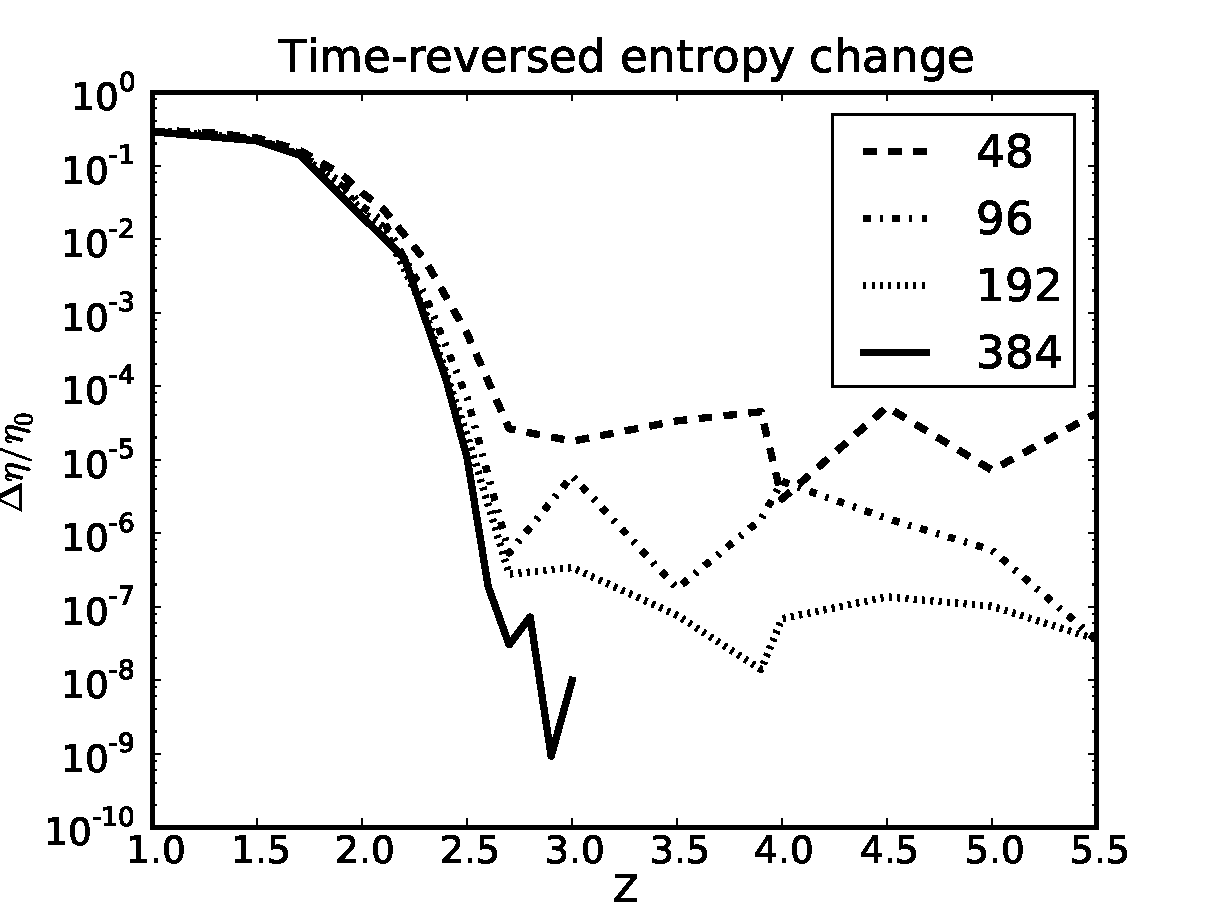
\includegraphics[width=7cm]{figures/trent_all.pdf} \end{center}
\end{frame}

\section{Generalizations}
\begin{frame}{Generalizations}
How general is this phenomenon?  Is it generic for
\begin{itemize}
  \item Different nonlinearities?
  \item Different materials?
  \item More general hyperbolic systems?
\end{itemize}
\end{frame}


\begin{frame}{Different Media}
\begin{columns}
  \column{5cm}
\begin{center} \includegraphics[width=5cm]{figures/sinoton_closeup.eps}

Sinusoidally varying medium \end{center}
  \column{5cm}
\begin{center} \includegraphics[width=5cm]{figures/3layer_stegoton.eps}

Three-layer medium \end{center}
\end{columns}
\end{frame}

\begin{frame}{Different Nonlinearities}
\begin{columns}
  \column{5cm}
  Cubic nonlinearity:
  $$\sigma(\epsilon,x) = K_1(x)\epsilon + K_3(x)\epsilon^3$$
  \includegraphics[width=5cm]{figures/cubic_steg.png}
  \column{5cm}
  Isothermal gas:
  $$\sigma(\epsilon,x) = -\kappa(x)/\epsilon^2$$
  $$\rho(x)=1$$
  \includegraphics[width=5cm]{figures/psys_steg.png}
\end{columns}
\end{frame}


\begin{frame}{Randomly perturbed media}
  Near-periodic medium with randomly perturbed interface locations 
\begin{columns}
  \column{5cm}
  \begin{center}  \includegraphics[width=5cm]{figures/random_steg_1percent.png}\\
  Perturbed by 1\%
  \end{center}
  \column{5cm}
  \begin{center}  \includegraphics[width=5cm]{figures/random_steg_10percent.png} \\
  Perturbed by 10\%\end{center}
\end{columns}
\end{frame}

\begin{frame}{Randomly perturbed media}
  Near-periodic medium with randomly perturbed piecewise constant coefficients 
\begin{columns}
  \column{5cm}
  \begin{center}  \includegraphics[width=5cm]{figures/random_steg_val_1percent.png}\\
  Perturbed by 1\%
  \end{center}
  \column{5cm}
  \begin{center}  \includegraphics[width=5cm]{figures/random_steg_val_25percent.png} \\
  Perturbed by 25\%\end{center}
\end{columns}
\end{frame}


\begin{frame} \frametitle{Stability in higher dimensions}
\begin{figure} \includegraphics[width=4.5in]{stegoton_evolution} \end{figure}
\end{frame}


\begin{frame} \frametitle{Summary of Main Points}
\begin{itemize}
  \item Entropy evolution and time-reversibility allow us to measure the
        formation of shocks in nonlinear wave simulations
  \item Periodic materials with high impedance contrast appear to 
        suppress the formation of shocks
  \item Large-amplitude signals in such materials can travel long
        distances without information loss
  \item Studying this phenomenon can also tell us new things about our
        numerical methods
\end{itemize}
\end{frame}


\begin{frame} \frametitle{Experimental Realization: Optical Stegotons?}
\begin{itemize}
    \item Medium consists of alternating layers of air and some material
            with high index of refraction and low loss
    \item High intensity laser pulse
    \item Currently we are designing simulations to test feasible
            design parameters
\end{itemize}
Joint work with Boon Ooi (KAUST).
\end{frame}

\end{document}
